\newcommand{\usecase}[5]{{
	\setlength\extrarowheight{5pt}
	\begin{tabular}{|p{3cm}|p{10cm}|}
		\hline
		Actor & #1\\
		\hline
		Entry conditions & #2\\
		\hline
		Event flow & #3\\
		\hline
		Exit condition & #4\\
		\hline
		Exceptions & #5\\
		\hline
	\end{tabular}
}}

\chapter{Specific Requirements}

\section{Use Case Diagrams}
Here are displayed the most important use case diagrams for the various actors.

\begin{figure}[h]
\centering
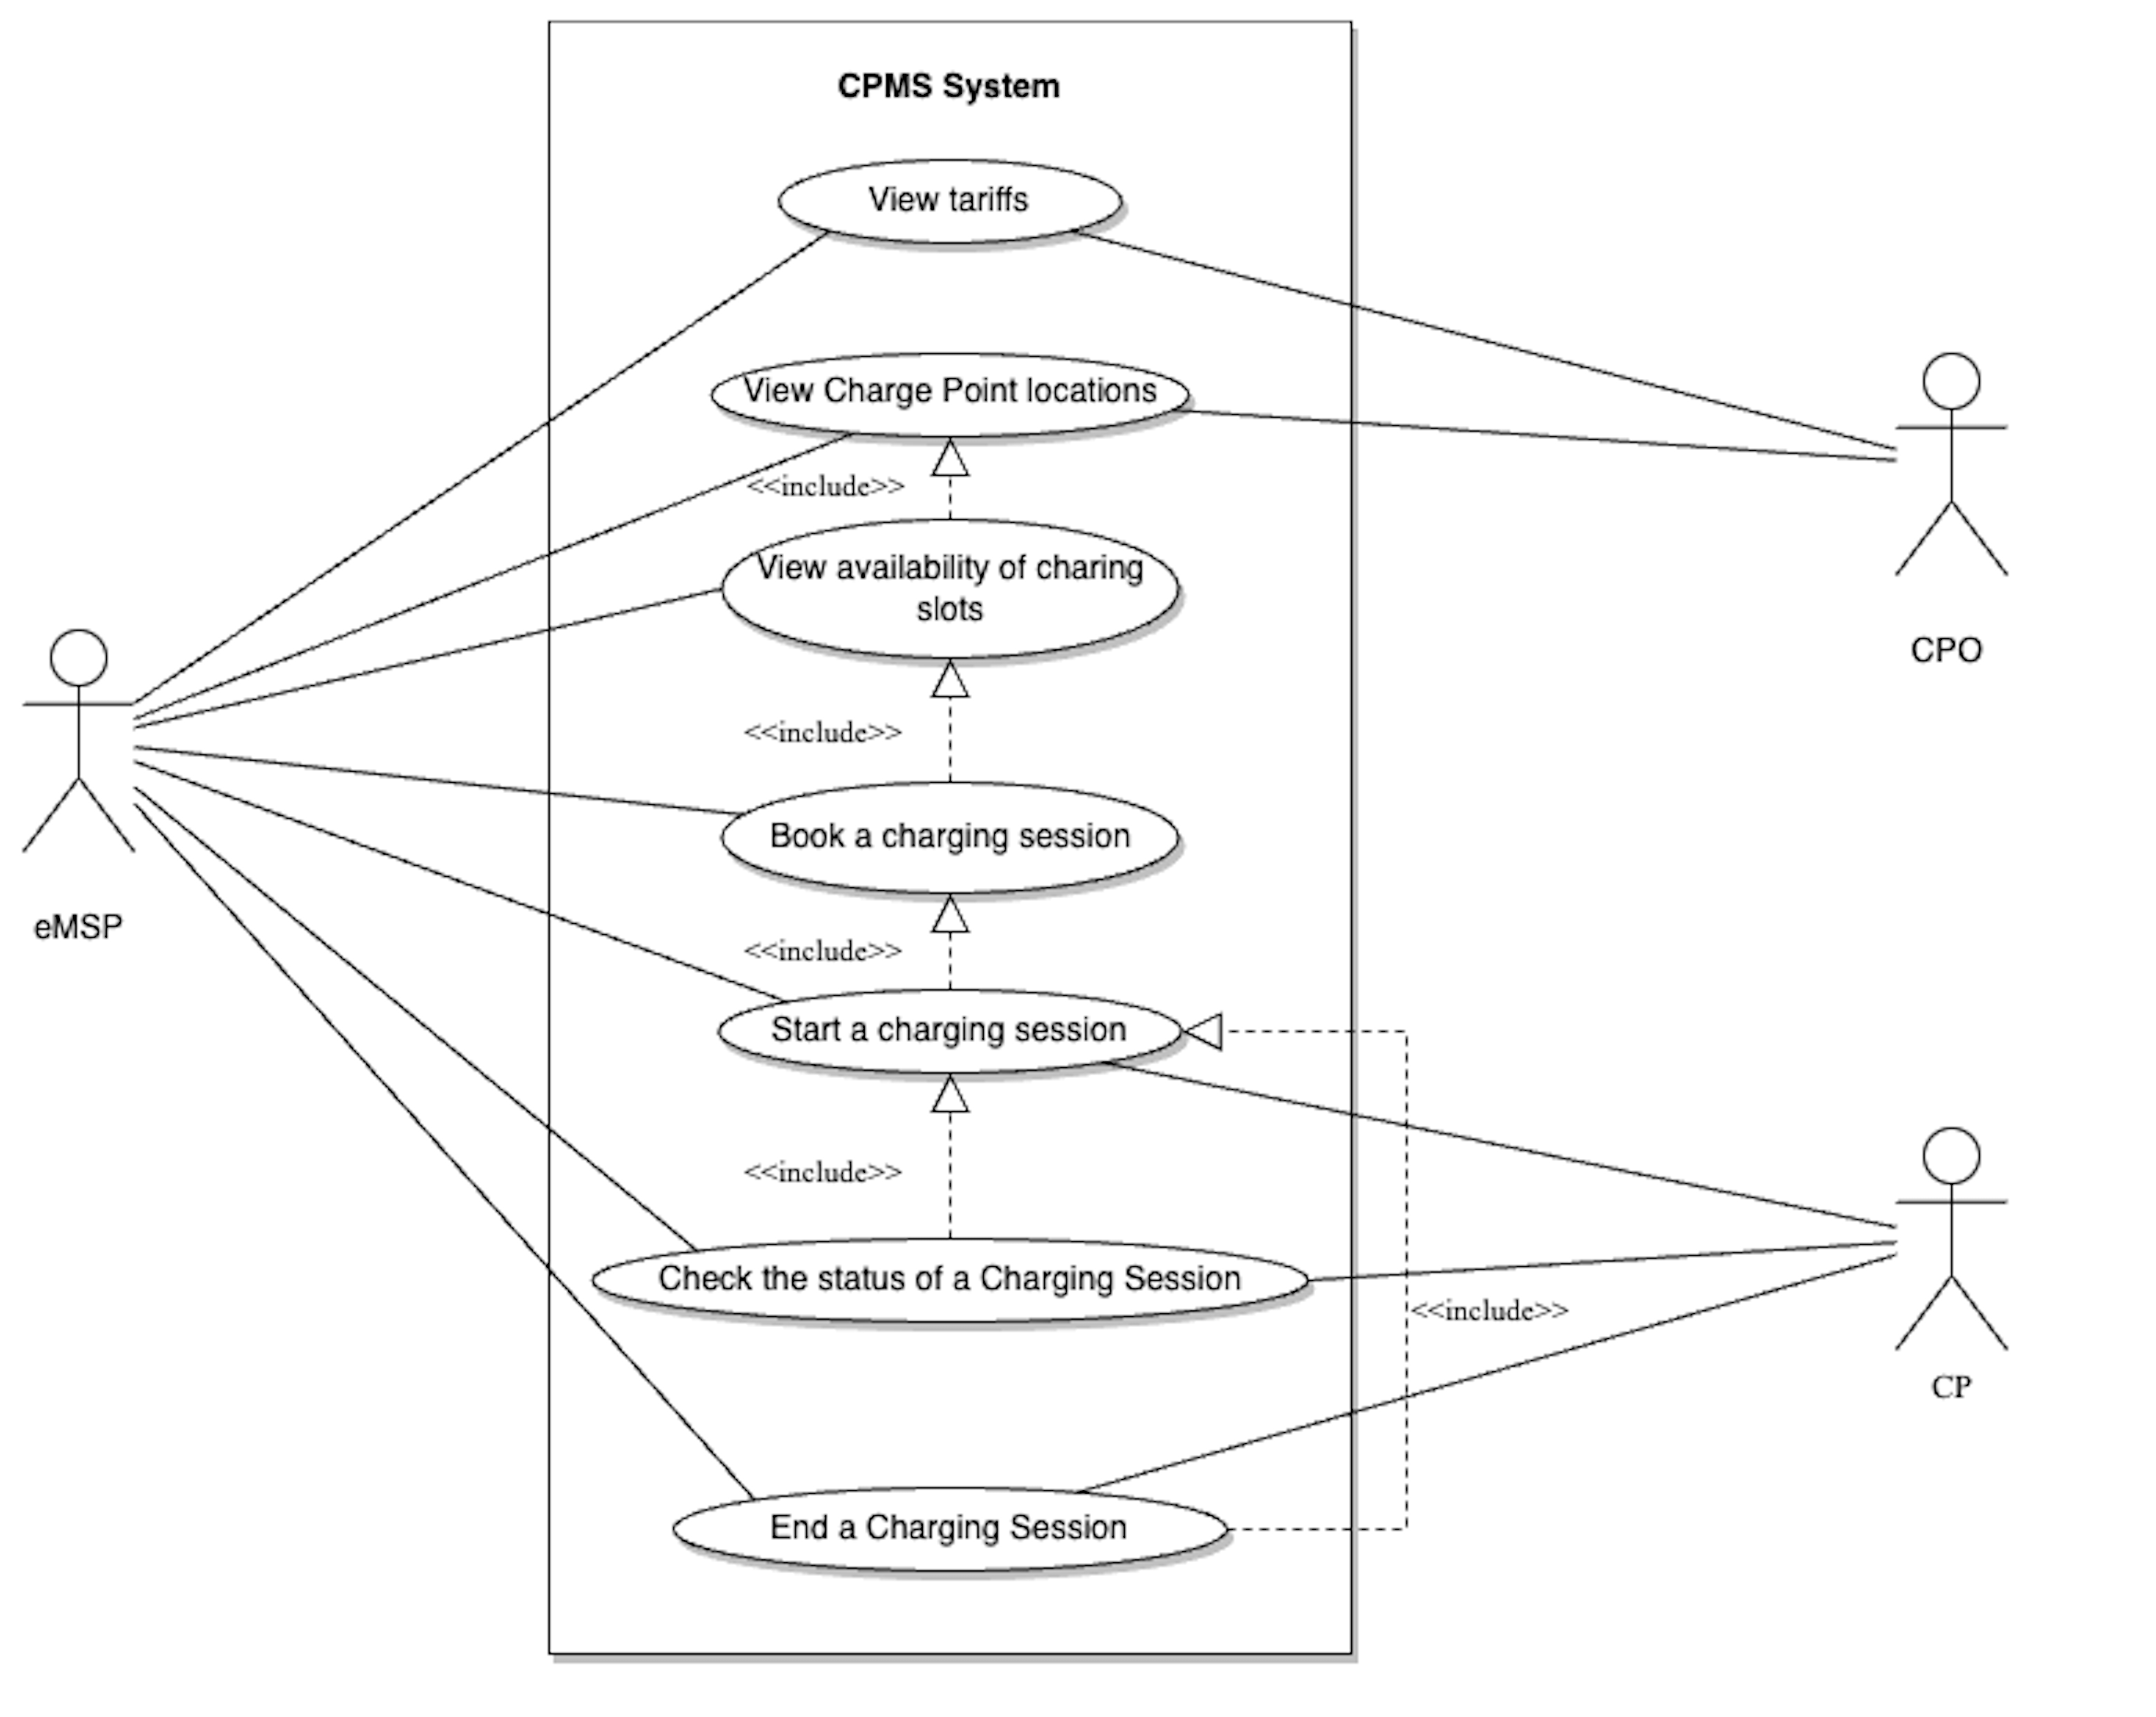
\includegraphics[width=8cm]{eMSP_usecase}
\caption{Use case diagram for eMSP}
\end{figure}


\begin{figure}[h]
\centering
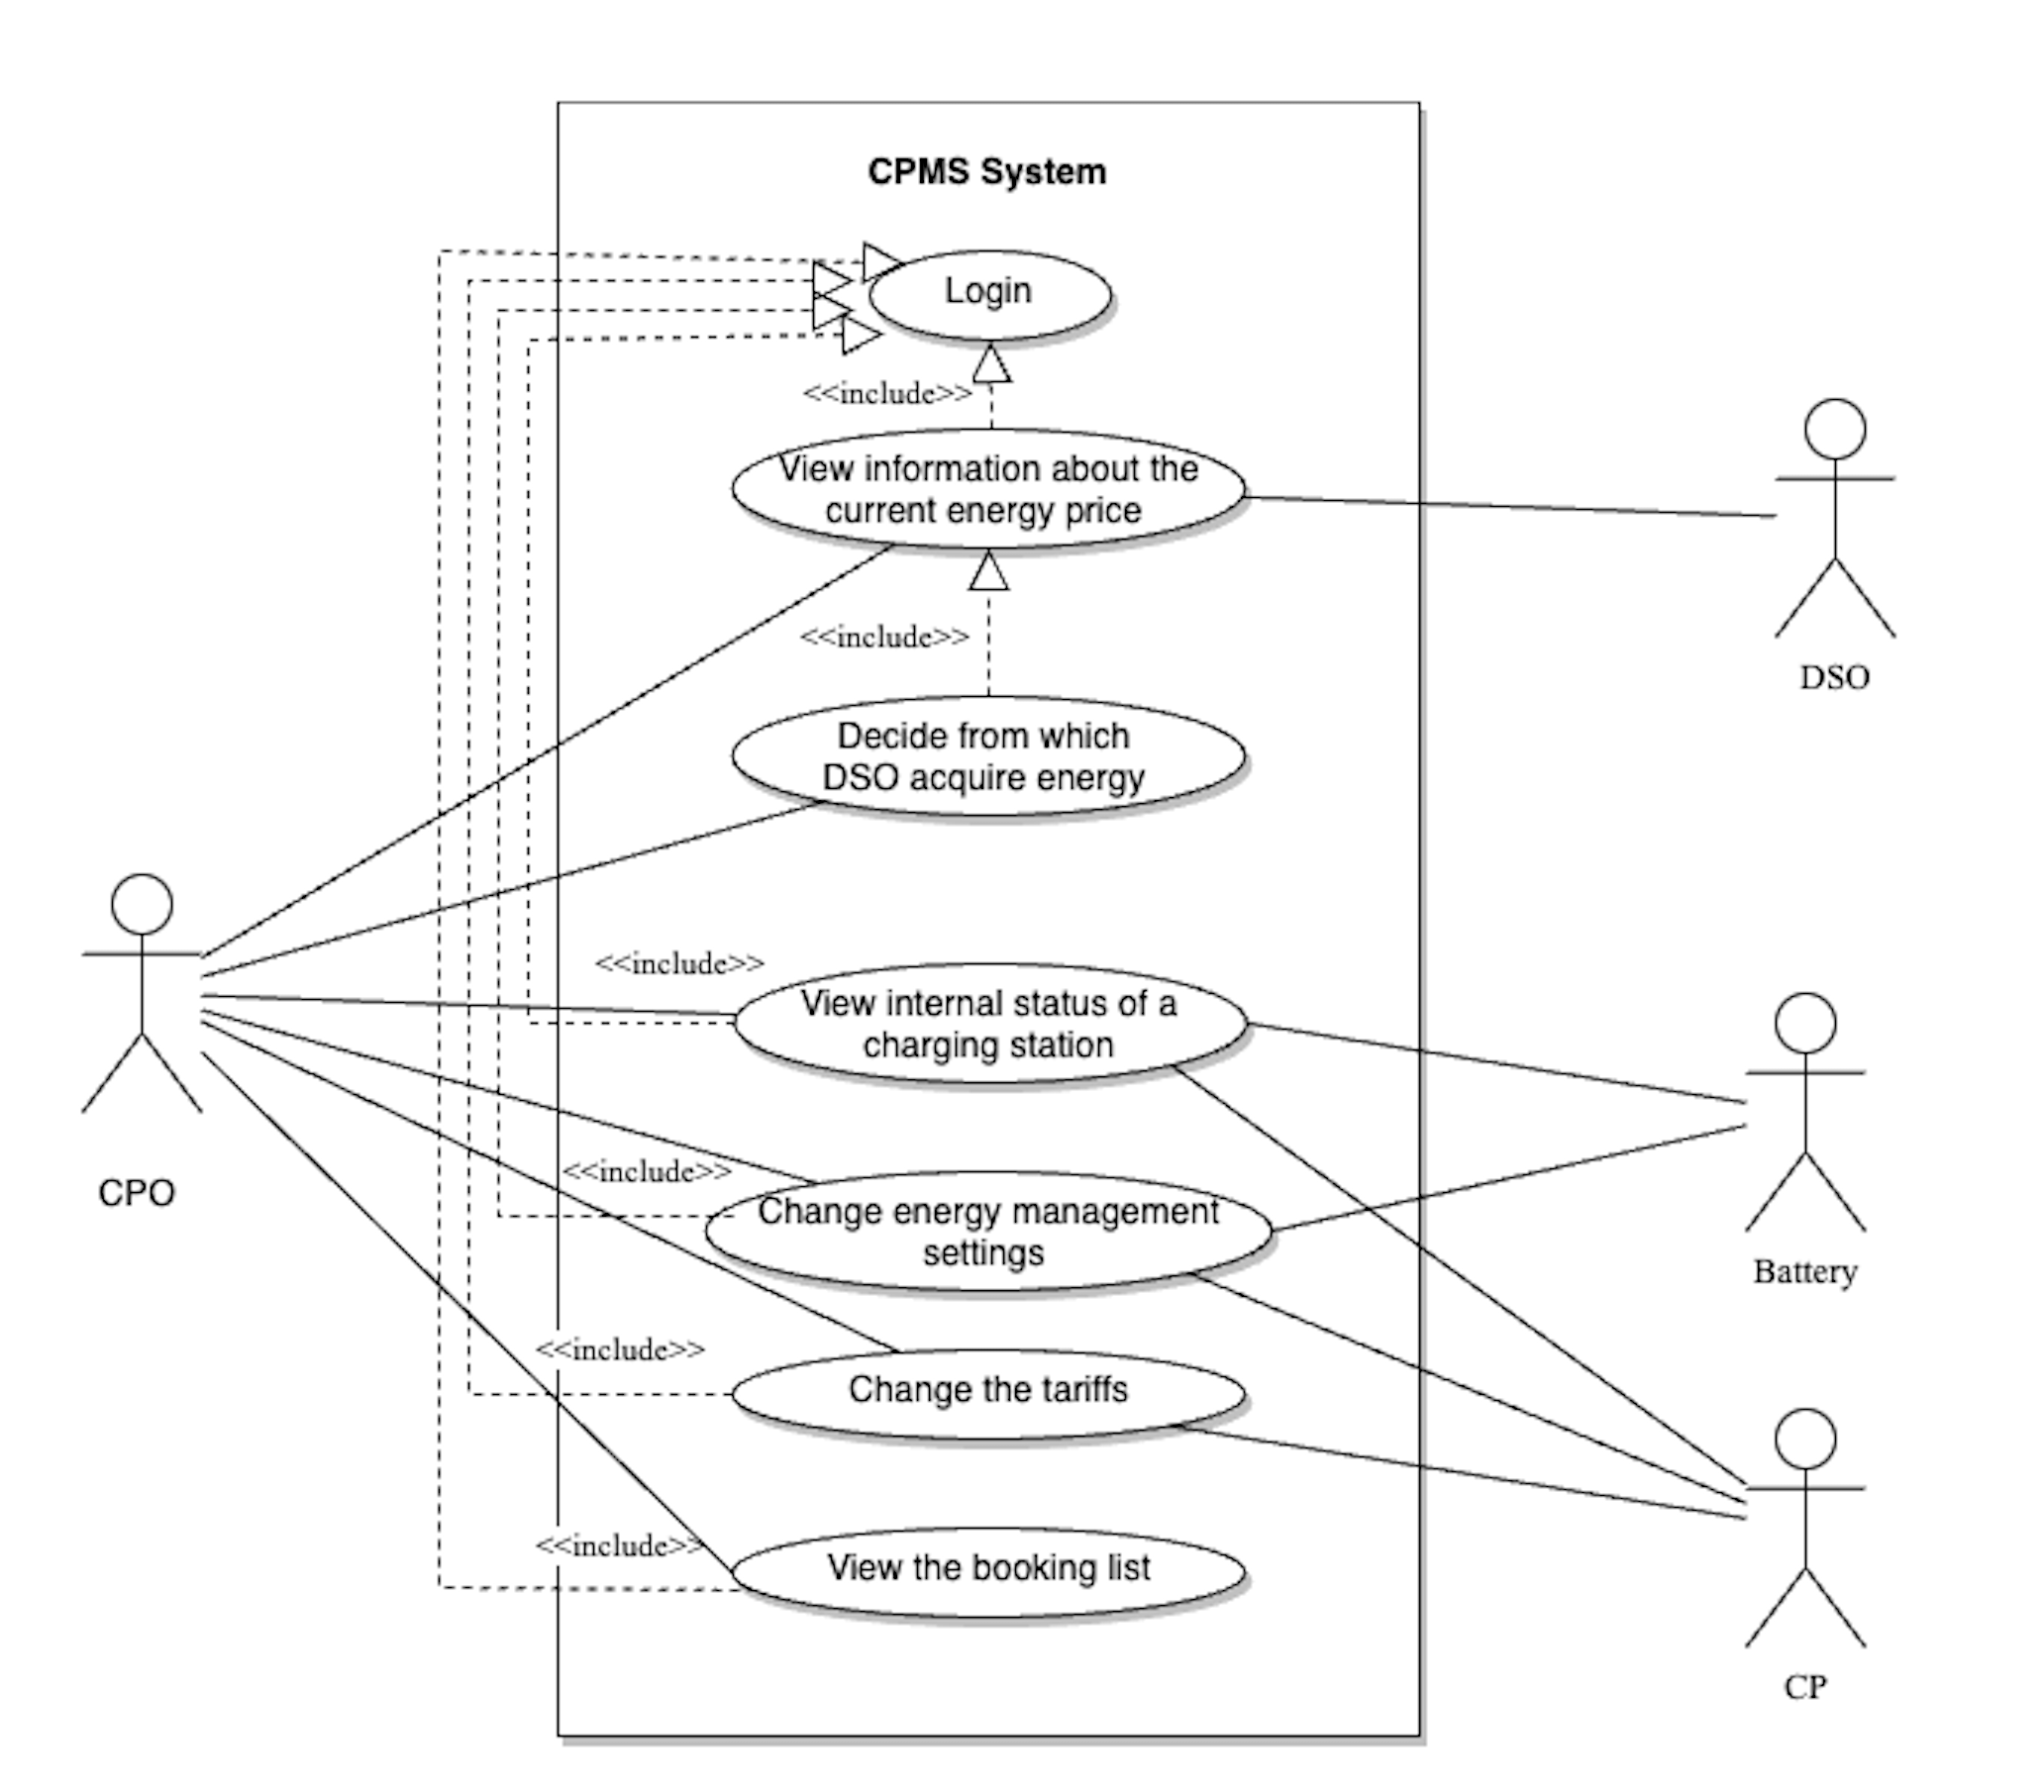
\includegraphics[width=\textwidth]{CPO_usecase}
\caption{Use case diagram for an CPO}
\end{figure}



\clearpage


\section{Use Cases}

\begin{enumerate}
	\descitem{CPO login}
	\usecase{CPO admin}
	{The CPO is registered into the system bus has to log in}
	{
	\begin{enumerate}[1.]
	\item The admin open the web portal of the CPMS
	\item The admin taps the "LogIn" button 
	\item The admin fills up the form
	\item The system validates the data and grants access to the admin
	\item The system redirect the admin to the main page
	\end{enumerate}
	}
	{The admin is logged in}
	{
	\begin{enumerate}[1.]
	\item The form data are incomplete or not valid 
	\item The system cannot process the data
	\end{enumerate}
	}
	
	
	\descitem{View information about energy price}
	\usecase{CPO admin, DSOs}
	{The admin is logged in }
	{
	\begin{enumerate}[1.]
	\item The admin taps on the "View energy prices" button 
	\item The system request to DSOs informations 
	\item The system shows the list of prices proposed by the various DSOs, also indicating the type of energy
	\end{enumerate}
	}
	{The admin goes yo another section or close the page }
	{
	\begin{enumerate}[1.]
	\item The system is unavailable
	\item Some or all of the DSOs are unavailable or unreachable
	\end{enumerate}
	}
	
	
	\descitem{CPO Change energy management settings }
	\usecase{CPO admin }
	{The admin is logged in}
	{
	\begin{enumerate}[1.]
	\item The admin select the charging station from the list
	\item The admin taps on the "Energy management" button
	\item The system shows a page with all the information on the current energy management
	\item The admin taps on the "Modify" button
	\item The system shows a page with all the parameters that the CPO can modify
	\item The admin modifies the parameters
	\item The admin taps on the "Save" button
	\end{enumerate}
	}
	{The admin goes yo another section or close the page }
	{
	\begin{enumerate}[1.]
	\item The system is unavailable
	\item Some or all of the DSOs are unavailable or unreachable
	\end{enumerate}
	}
	
	
	\descitem{Displays information about the internal status of a charging station}
	\usecase{CPO admin }
	{The admin is logged in }
	{
	\begin{enumerate}[1.]
	\item The admin select the charging station from the list
	\item The admin taps on the "System monitor" button
	\item The system shows a page with all the information about the charging station status
	\end{enumerate}
	}
	{The admin goes yo another section or close the page}
	{
	\begin{enumerate}[1.]
	\item The system is unavailable
	\end{enumerate}
	}
	
	\descitem{Start a Charging session}
	\usecase{eMSP, Charging point}
	{The charging slot has been booked}
	{
	\begin{enumerate}[1.]
	\item The system receives the command from the eMSP
	\item The system verifies the validity of the reservation
	\item The system sends the command to the charging slot
	\item The system sends the confirmation to the eMSP
	\end{enumerate}
	}
	{eMSP receive a response}
	{
	\begin{enumerate}[1.]
	\item The charging slot is unreachable
	\item The system does not confirm the reservation
	\item The charging slot does not confirm activation
	\end{enumerate}
	}
	
	\descitem{End a charging session}
	\usecase{eMSP, CS }
	{There is a active session }
	{
	\begin{enumerate}[1.]
	\item The system receives the request to end the session from the eMSP
	\item The system sends the request to end the session to the CS
	\item The system receives the end session confirmation from the CS
	\item The system send the confirm to the eMSP
	\end{enumerate}
	}
	{eMSP receives a response}
	{
	\begin{enumerate}[1.]
	\item The CS is unreachable
	\item The CS cannot end the session
	\item eMSP cannot receive the response
	\end{enumerate}
	}
	
	\descitem{Update the state of the charging session}
	\usecase{eMSP, CS }
	{There is a active session }
	{
	\begin{enumerate}[1.]
	\item The system receives information about the status of the charging session from the CS
	\item The system sends information about the status of the charging session to the eMSP
	\end{enumerate}
	}
	{eMSP receives information about the status of the charging session}
	{
	\begin{enumerate}[1.]
	\item eMSP is unreachable
	\item The CS cannot reach the system
	\end{enumerate}
	}
	
	
\end{enumerate}
\clearpage
\newpage

\section{Sequence Diagrams}
Here are presented the sequence diagrams for the most important use cases.Only the "success" flow is displayed, every exception in the communication flow results in an error message displayed to the log file and a request retry.\\

\begin{figure}[h]
\centering
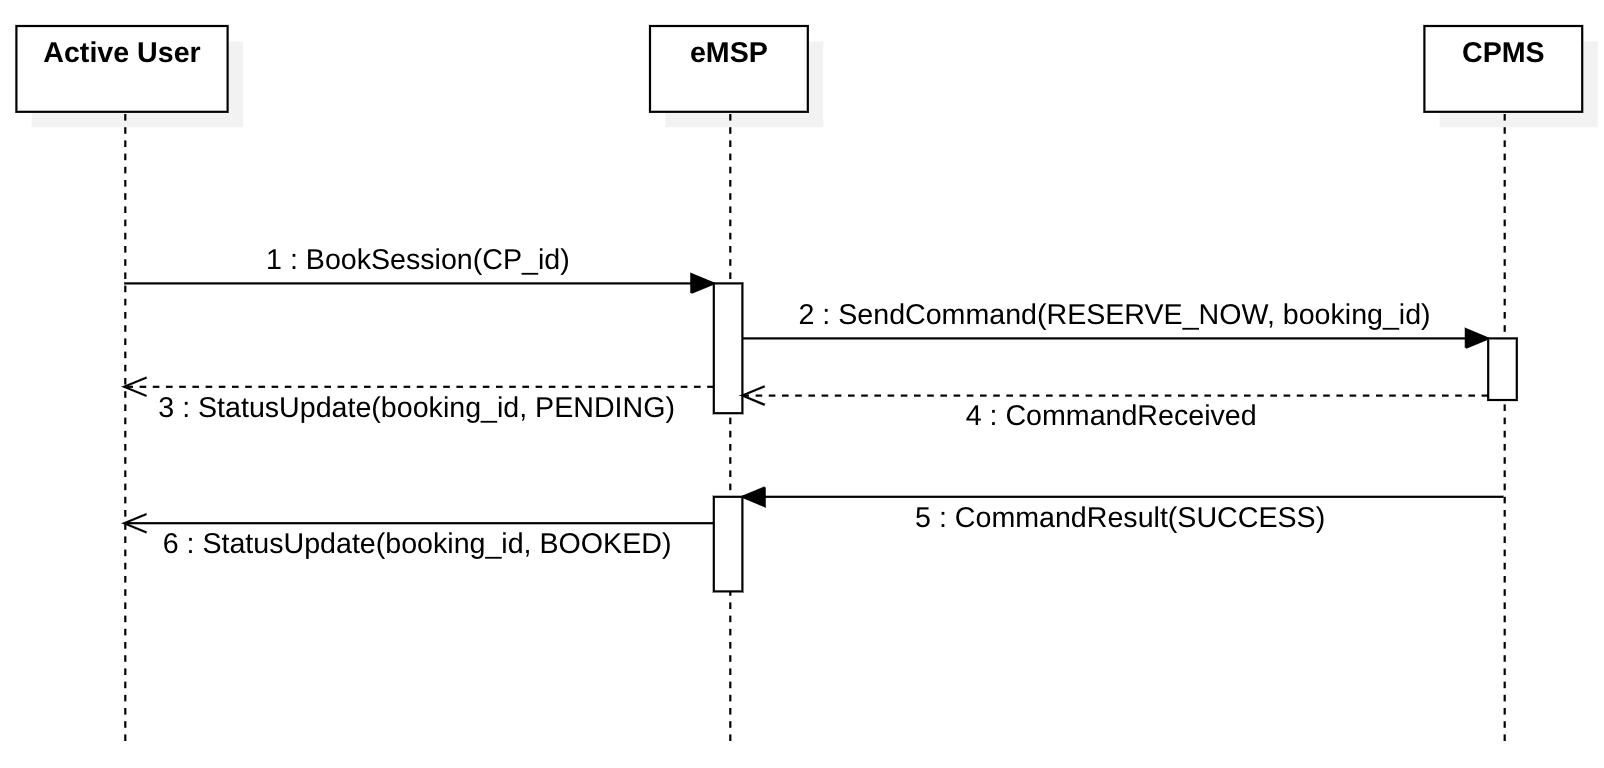
\includegraphics[width=13cm\textwidth]{sequence_diagrams/book_session}
\caption{Sequence diagram for the booking process of a new charging session}
\end{figure}


\begin{figure}[h]
\centering
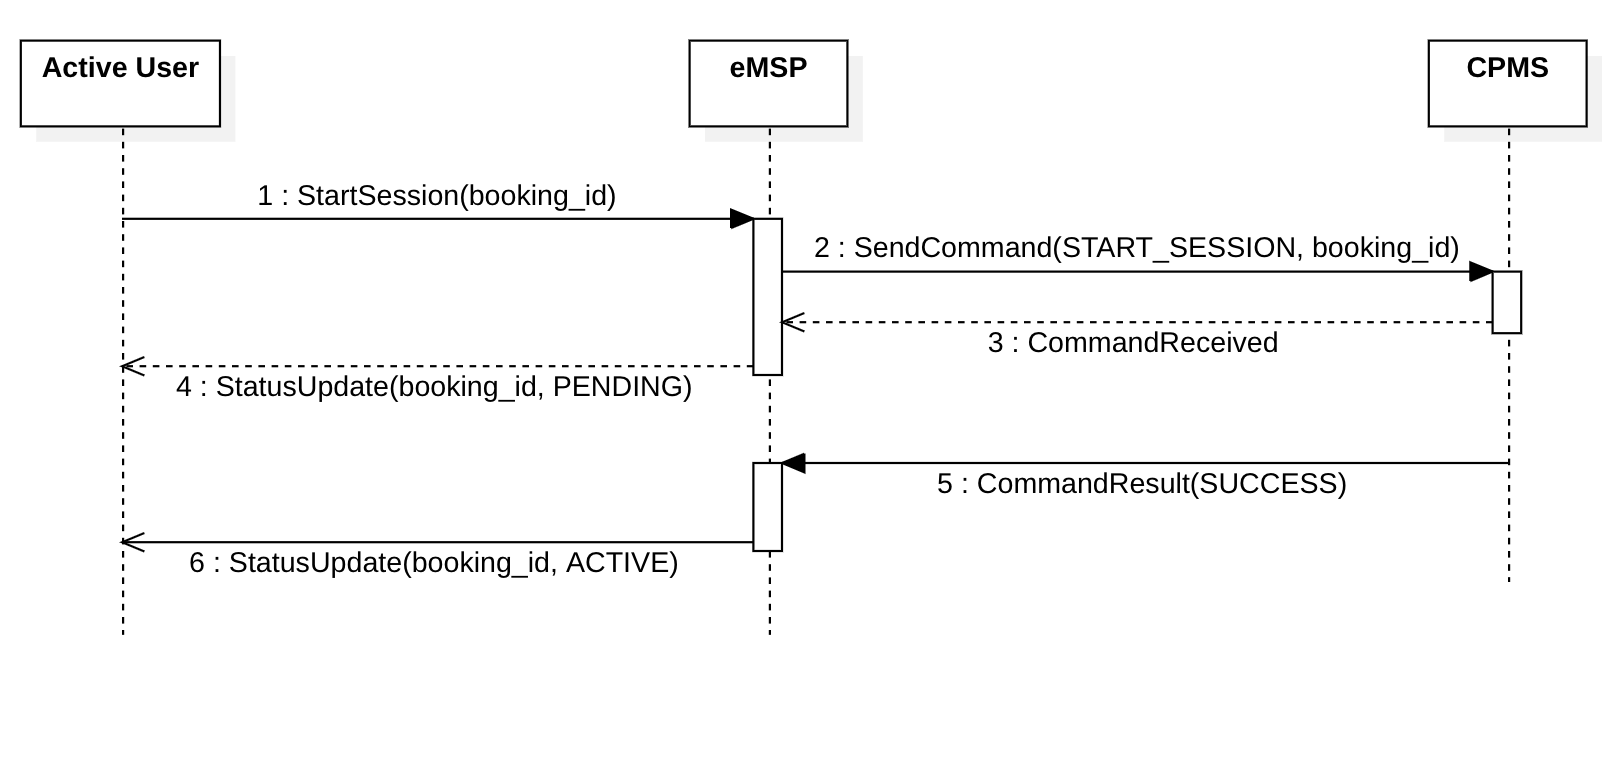
\includegraphics[width=13cm\textwidth]{sequence_diagrams/start_session}
\caption{Sequence diagram for the starting of a charging session}
\end{figure}


\begin{figure}[h]
\centering
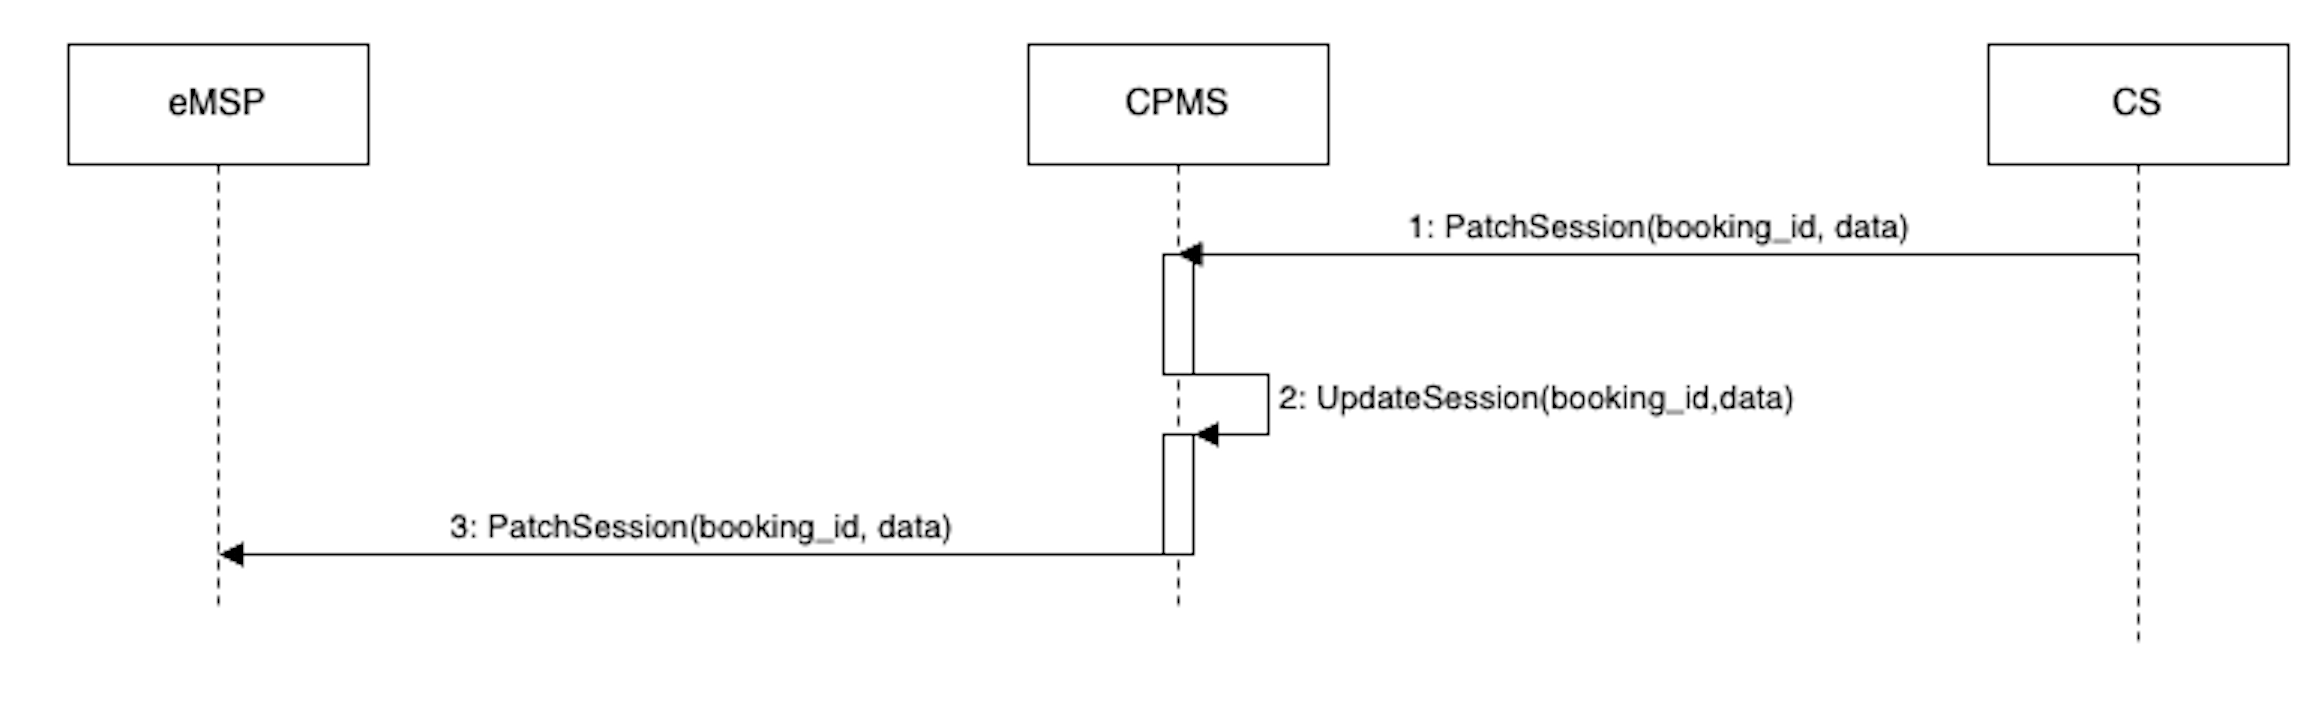
\includegraphics[width=13cm\textwidth]{sequence_diagrams/state_session}
\caption{Sequence diagram for the notification of a charging session state }
\end{figure}


\begin{figure}[h]
\centering
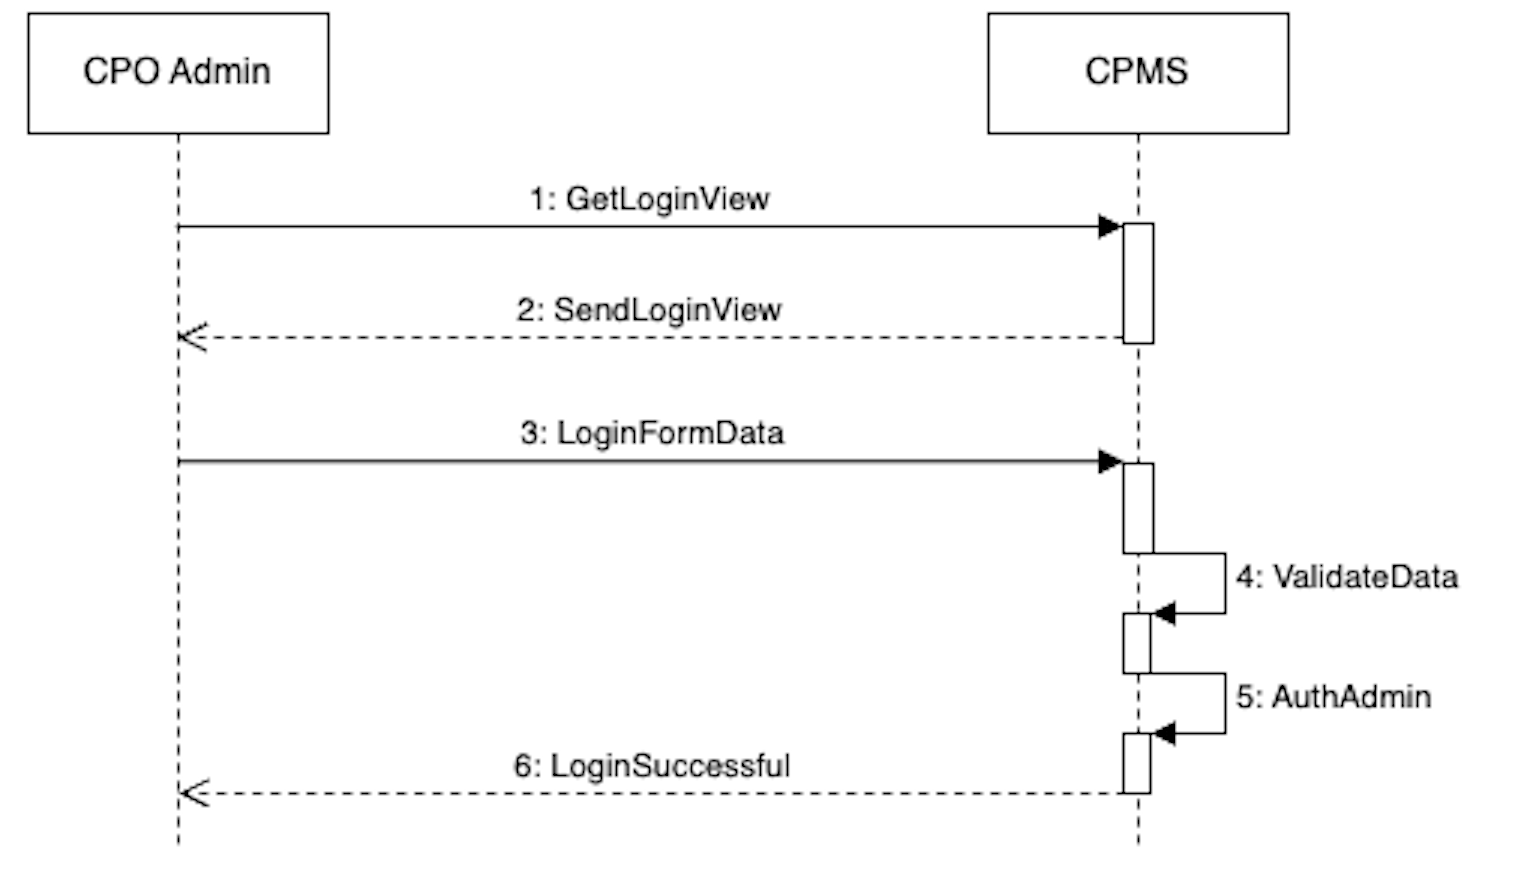
\includegraphics[width=13cm\textwidth]{sequence_diagrams/energy_settings}
\caption{Sequence diagram for the change of energy management settings}
\end{figure}

\clearpage
\newpage


\section{Functional Requirements}

The system should:\\

\begin{tabular}{|c|l|}
	\hline
	\bf{Requirement} & \bf{Description} \\
	\hline
	R1 & Allow to book a charging session on a specific CS\\
	\hline
	R2 & Allow to start a charging session on a specific CS\\
	\hline
	R3 & Allow to stop a charging session on a specific CS\\
	\hline
	R4 & Forward information about the state of a charging session to the eMSP\\
	\hline
	R5 & Allow Login for CPO\\
	\hline
	R6 & Allow to view information about the internal status of a charging station\\
	\hline
	R7 & Forward of the offered tariffs\\
	\hline
	R8 & Allow CPO to set or change tariffs\\
	\hline
	R9 & Allow CPO to enter static information about charging stations\\
	\hline
	R10 & Forward information about the location of charging stations\\
	\hline
	R11 & Forward information about the location of charging stations\\
	\hline
	R12 & Allow CPOs to change the settings and management settings of the charging station\\
	\hline
\end{tabular}

\subsection{Requirements mapping on Goals}
\begin{tabular}{|c|l|}
	\hline
	\bf{Goal} & \bf{Requirements}\\
	\hline
	G1 & R1, R2, R3\\
	G2 & R1, R2, R3, R4,\\
	G3 & R5, R6\\
	G4 & R5, R7, R8\\
	G5 & R9, R10\\
	G6 & R11\\
	G7 & R5, R12\\
	G8 & R5, R12\\
	G9 & R5, R12\\
	\hline
\end{tabular}

\clearpage
\newpage

\section{Performance Requirements}
As most of the Charge Points are located in the city centre, where internet connectivity is usually optimal and at high speed, the system does not have special requirements for performances related to bandwidth usage. Also, no particular usage spikes are expected at any moment, so server load should be directly connected to the number of users and Charge Points covered by the system.

\section{Design Constraints}
\subsection{Standards compliance}
For the legal aspect it is necessary to follow the requirements of the GDPR regarding the management of sensitive data of users and CPOs. While to allow interconnection with the different eMSPs and CPs, it is necessary to follow the OCPI and OCPP standards in the implementation of communication protocols and data structures.

\subsection{Hardware limitations}
No particular hardware are required to use the System.

\section{Non-functional Requirements}

{
\setlength\extrarowheight{5pt}
\begin{tabular}{|p{3cm}|p{10cm}|}
	\hline
	NFR1 & Reliability impacts the system usage and the related business, to keep it as high as possible, fall back servers shall be considered while designing the infrastructure.\\
	\hline
	NFR2 & Availability also has a huge impact but as this is not a sensible service that needs to be up and running at all time, a good compromise with cost effectiveness can be considered.\\
	\hline
	NFR3 & The basic security standard "defacto" measurements should be followed, SSL and HTTPS should be enough to offer both security and ease to use.\\
	\hline
\end{tabular}
}

\clearpage
\newpage



\section{External Interface Requirements}
\subsection{User Interfaces}
The CPO's user interface can be accessed via a web portal that can be used on any device with an internet connection and a web browser.

\subsection{Hardware interfaces}
There are no hardware interfaces

\subsection{Communication interfaces}
As the system needs to communicate with multiple actors, the following communication interfaces are required:

\begin{enumerate}
	\descitem{CPMS communication:}
	To share data with the various eMSPs, an active, low-latency internet connection is needed. Also is required that the eMSP follows the OCPI protocol.\\
   
   \descitem{CS communication:} 
    To share data with the various CPs, an active, low-latency internet connection is needed. Also is required that the eMSP follows the OCPP protocol.
\end{enumerate}
